\subsection{Choice of the circuit topology}

A specified for this assignment we need to design a:

\textit{Low-power supply-scalable (0.7-1.0V) I/O Link operating at 2-10Gb/s with at
least 2-tap voltage-mode TX. Minimize energy efficiency of the link, with an upper target
of 1pJ/b at 10Gb/s. }

So for the TX driver we first of all need to design a VM driver, for this we've chosen to use a slice topology in order to obtain a differential TX driver with equalization and tunable impedance. To aid in the impedance tuning and lowering the power consumption we also seek to implement a shunt as well (this isn't included in the schematic in Cadence yet!), the shunt we seek to implement will be a tunable shunt, such that we can use fewer slices in the TX driver. Using less slices should help lowering the load for the pre-drivers and as such lower the total power consumption.

So for the TX driver we've decided to design for the topology depicted in figure \ref{fig:topology_tx}, where the serializer is responsible for serializing the input data to the transmitter, the two signals on each bus from the serializer to the TX driver is the cursor and the first post-cursor, the post-cursor is needed for serialization. The clock is a half-rate clock and thus it has two lines to the driver and serializer. The TX driver is as mentioned a slice design, where we've decided on using 12 slices in total, 9 for the cursor and 3 slices for the post-cursor. The reason we've decided to split up the allocation of slices is that this will lower the load for the pre-drivers.

\begin{figure}[H]
  \centering
  {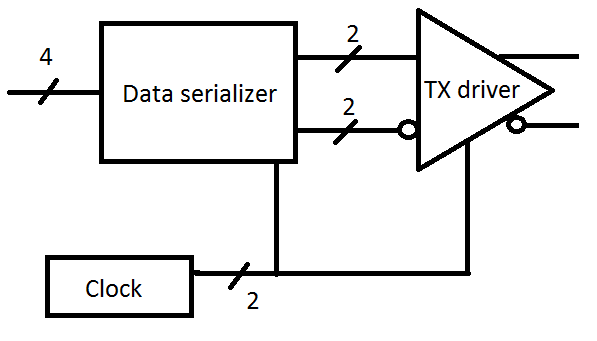
\includegraphics[scale=0.55]{img/topology_tx.png}}
  \caption{Transmitter top level topology}
  \label{fig:topology_tx}
\end{figure}

The topology design is based on the half-rate transmitter design from ~\cite{menolfi2007a}, also depicted in figure \ref{fig:topology1}, we will however only feature one tap with a known sign, which will result in a simpler architecture.

\begin{figure}[H]
  \centering
  {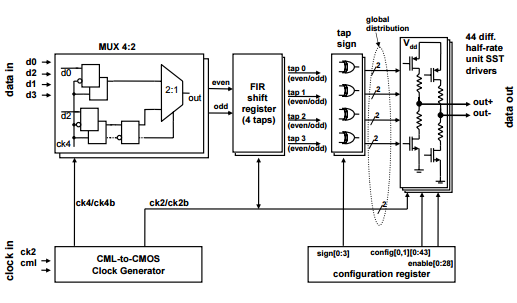
\includegraphics[scale=0.55]{img/topology_tx1.png}}
  \caption{Transmitter top level topology from ~\cite{menolfi2007a}}
  \label{fig:topology1}
\end{figure}


The slice design we're going to use is based on the design used in ~\cite{menolfi2007a}, also depicted in figure \ref{fig:topology0}, as this is a slice designed for half-rate clocking operation hence very fitting to the design choices we made earlier.

\begin{figure}[H]
  \centering
  {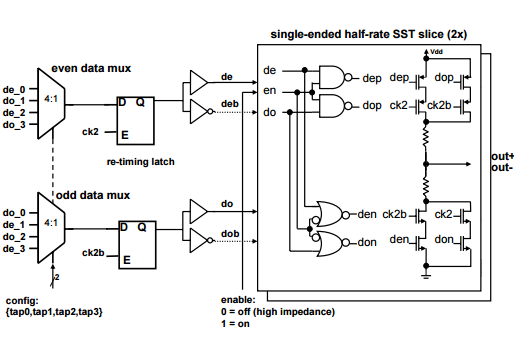
\includegraphics[scale=0.55]{img/topology_tx0.png}}
  \caption{Half-rate slice topology from ~\cite{menolfi2007a}}
  \label{fig:topology0}
\end{figure}

For the serializer we haven't decided upon a final design, as we are uncertain about how the data will be presented to the transmitter, this will however be decided in future work.